% Бүлэг 3

\chapter{... системийн зохиомж ба хөгжүүлэлт} % Зарим нэг зөвлөмж
\label{Chapter3} % Энэ бүлэг рүү ишлэл хийх бол \ref{Chapter2} командыг ашигла 

\section{Системийн архитектур}
\paragraph{} 
Зургаас объект илрүүлэлт хийдэг веб систем нь Back-end болон Front-end гэсэн үндсэн хоёр хэсгээс бүрдэнэ. Зураг \ref{fig:sys-arch} -д үзүүлсний дагуу Front-end хэсэг нь хэрэглэгчид харагдаж, хэрэглэгчтэй харилцах хэсэг бөгөөд хэрэглэгчийн оролтын мэдээллийг авч Back-end хэсгээс гаргасан сервисийг ашиглан Back-end хэсэг рүү хүсэлт явуулж, хариуг аван хэрэглэгчийг гаралтын мэдээллээр хангана. Back-end хэсгийн хувьд системийн логик үйл ажиллагааг хангаж ажилладаг. Хэрэглэгчийн нэвтрэлт, бүртгэл, объект илрүүлэлттэй холбоотой сервисүүдийг гаргаж, монгол хэл дээрх текстийг аудио руу хөрвүүлж өгөх 3-дагч талын сервис болох ChimegeAPI, хэрэглэгчдийн мэдээлэл болон тэдгээрт хамааралтай объект илрүүлэлтэд ашигласан файлын мэдээллийг хадгалах MySQL өгөгдлийн сантай ажиллана.   
\begin{figure}[H]
    \centering
    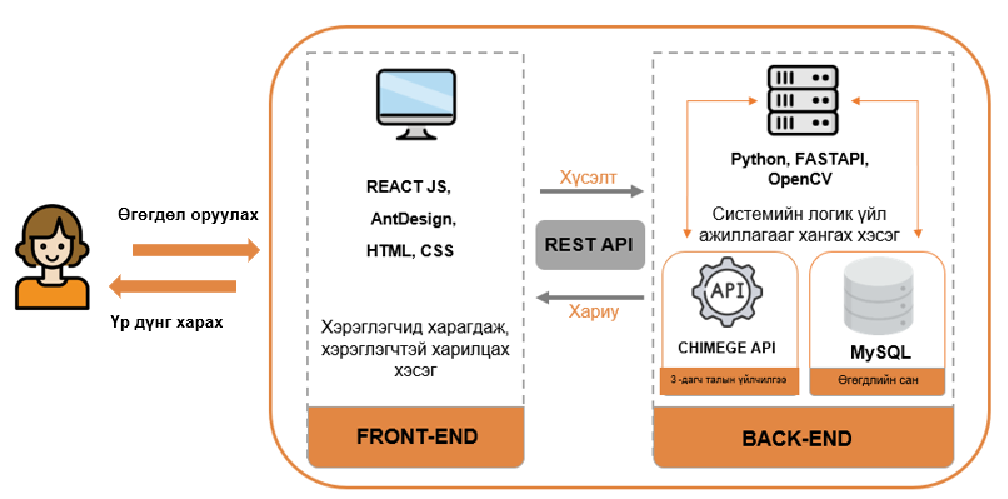
\includegraphics[scale=0.9]{Figures/chapter3/arch-diagram.pdf}
    \caption{Системийн архитектур}
    \label{fig:sys-arch}
\end{figure}
	

\section{Зохиомжийн шатны класс диаграмм}
\paragraph{} Объект илрүүлэлт хийдэг веб системийн зохиомжийн шатны класс диаграммд \say{control} төрлийн \say{Хэрэглэгч}, \say{Үр дүнгийн боловсруулалт}, \say{Хэлний төрөл}, \say{Хэрэглэгчийн файл} , \say{Объект илрүүлэлт}, \say{Бүртгэл} гэсэн 6-н класс ,\say{entity}төрлийн \say{Хэрэглэгчийн файлын мэдээлэл}, \say{Хэрэглэгчийн мэдээлэл} гэх 2 класс, \say{boundary} төрлийн \say{Объект илрүүлэлтийн дэлгэц},\say{Бүртгэлийн дэлгэц}, \say{ОТР шалгах дэлгэц}, \say{Хэрэглэгчийн файлын мэдээллийн дэлгэц}, \say{Хэрэглэгчийн мэдээллийн дэлгэц} гэсэн 5-н класс буюу нийт 13 классын аттрибут болон операторуудыг тодорхойлсон. Зураг \ref{fig:z-class} -д тэдгээр классуудын стерео төрлийг тодорхойлж, класс хоорондын холбоо хамаарлыг ассосиэйшн болон бүрдмэл холбоо хамаарлаар дүрсэлж, зарим класс хоорондын холбоо хамааралд ашиглалтын хараат байдлыг дүрсэлсэн.
\begin{figure}[!h]
    \centering
    \includegraphics[scale=0.4, angle = 90]{Figures/chapter3/s_class_diagram.jpg}
    \caption{Класс диаграмм}
    \label{fig:z-class}
\end{figure}	


\section{Өгөгдлийн ерөнхий схем }
\paragraph{} Объект илрүүлэлт хийдэг веб системийн өгөгдлийн сан нь хэрэглэгч болон хэрэглэгчийн файл гэсэн хоёр хүснэгтийг агуулна. Хэрэглэгч хүснэгт нь системд бүртгүүлсэн хэрэглэгчдийн овог нэр, имейл, нууц үг болон хэрэглэгчийн кодыг анхдагч түлхүүрээр хадгална. Хэрэглэгчийн файл хүснэгт нь файлын нэр, локал сервер дээр хадгалагдсан байршил, текст, аудио мэдээлэл, огноо, хэрэглэгчийн кодыг гадаад түлхүүрээр, файлын кодыг анхдагч түлхүүрээр хадгална. Зураг \ref{fig:erd} -д системийн хөгжүүлэлтийн хүрээнд үүсгэсэн өгөгдлийн сангийн "Хэрэглэгч", "Хэрэглэгчийн файл" гэсэн хүснэгтүүд, тэдгээрийн аттрибутууд болон тэдгээр хүснэгтүүд "1 : олон" харьцаагаар дүрслэгдсэнийг харуулж байна. 
\begin{figure}[H]
    \centering
    \includegraphics[scale=0.8]{Figures/chapter3/erd.PNG}
    \caption{Өгөгдлийн ерөнхий схем}
    \label{fig:erd}
\end{figure}	

\section{Системийн прототип}
\paragraph{} Системийн үндсэн хуудас, бүртгүүлэх болон нэвтрэх хуудас, бүртгэлтэй хэрэглэгчийн мэдээллээ шинэчлэх болон файлын мэдээллүүдээ зохион байгуулах хуудаснуудын прототип загварыг дүрслэн харуулна.

\par \noindent Зураг \ref{fig: proto_obj_det} -д зургаас объект илрүүлэх вебийн хэрэглэгчийн бүртгэлээр ороогүй байх үеийн объект илрүүлэлт хийх нүүр хуудас харагдаж байна. 
\begin{figure}[!h]
    \centering
    \includegraphics[scale=0.305]{Figures/chapter3/Frame_1.pdf}
    \caption{Зургаас объект илрүүлэлт хийх хуудасны прототип}
    \label{fig: proto_obj_det}
\end{figure}
\newline
\par \noindent Зураг \ref{fig: proto_obj_det} -д үзүүлсэн хэрэглэгчийн бүртгэлээр нэвтрээгүй байх үеийн нүүр хуудасны толгой хэсэгт байрлах "Бүртгүүлэх" лабел -г дарснаар тус хуудас гарч ирнэ. Зураг \ref{fig:proto_signup} -д хэрэглэгчийн бүртгэлийн мэдээллийг авч бүртгэл үүсгэх хуудсыг харуулж байна.
\begin{figure}[H]
    \centering
    \includegraphics[scale=0.23]{Figures/chapter3/Frame_2.pdf}
    \caption{Бүртгэл үүсгэх хуудасны прототип}
    \label{fig:proto_signup}
\end{figure}


% \clearpage
\section{Хөгжүүлсэн системийн интерфейс}
\paragraph{} Хөгжүүлэгдсэн системийн объект илрүүлэлт хийх, нэвтрэх, бүртгүүлэх, ОТР шалгах хуудаснууд болон хэрэглэгчийн бүртгэлээр нэвтэрч орсон үеийн объект илрүүлэлт хийх хуудас , өөрт бүртгэлтэй зургуудын жагсаалт харах хуудасны интерфейсийг энэ хэсэгт тайлбарлана.


\par \noindent Зураг \ref{fig:home} -д харуулсан интерфейстэй хуудас нь хэрэглэгчийг веб хуудас руу хэрэглэгчийн бүртгэлгүйгээр хандах үед харагдана. Хуудасны зураг оруулах хэсэгт зургийг оруулснаар зургийн нэр доод хэсэгт харагдана. Англи болон монгол гэсэн сонголтуудаас хэлний сонголтоо хийгээд "Илрүүлэлт хийх" товчийг дарснаар текст болон аудио мэдээлэл хэсгүүдэд үр дүн харагдана. 

\begin{figure}[H]
    \centering
    \includegraphics[scale=0.4]{Figures/chapter3/home.pdf}
    \caption{Объект илрүүлэлт хийх хуудасны интерфейс}
    \label{fig:home}
\end{figure}
\par \noindent Зураг \ref{fig:login} -д системийн нэвтрэх хуудасны интерфейсийг харуулсан. Бүртгэлтэй хэрэглэгч имейл хаяг болон нууц үгээ оруулаад "Нэвтрэх" товчийг дарж системд нэвтэрнэ. Хэрэглэгчийн оруулсан имейл хаяг бүртгэлгүй эсвэл нууц үг буруу тохиолдолд алдааны мессежийг хэрэглэгчид харуулна. Хэрэв бүртгэлгүй бол "Одоо бүртгүүлэх" гэсэн лабелийг дарж бүртгүүлэх хуудас руу очиж болно.
\begin{figure}[H]
    \centering
    
\includegraphics[scale=0.4]{Figures/chapter3/login.pdf}
    \caption{Нэвтрэх хуудасны интерфейс}
    \label{fig:login}
\end{figure}

\section{Системд хийгдсэн тест}
%альфа бета тестүүд ямар хэмжээнд хийгдсэн талаар, хийгдсэн тестүүдийн талаар
\section{Системийн нэвтрүүлэлт}
%Системийг бодит хэрэглэгч дээр ямар хэмжээнд нэвтрүүлсэн талаар


\section{Бүлгийн дүгнэлт}
\paragraph{} Энэ бүлэгт ерөнхийдөө системийн зохиомжийг гаргасан. Системийн архитектур, класс диаграмм, дарааллын диаграмм, өгөгдлийн ерөнхий схем, системийн прототип загвар болон хөгжүүлэгдсэн системийн интерфейсийг багтаасан. Системийн архитектурыг front-end болон back-end гэсэн үндсэн 2 хэсэгт хувааж, тэдгээр хэсгүүд дээр хийгдэх үйл ажиллагаануудыг бүдүүвч байдлаар дүрсэлсэн. Ингэхдээ front-end хэсгийг хэрэглэгчид харагдаж, хэрэглэгчтэй харилцах хэсэг, back-end хэсгийг системийн логик үйл ажиллагааг хангах хэсэг гэж тодорхойлоод REST API ашиглан тэдгээрийн дунд холболт үүсгэхээр дүрсэлсэн. Класс диаграмм дээр шинжилгээний шатны control төрлийн 6-н класс дээр нэмээд boundary төрлийн 5-н класс, entity төрлийн 2 классыг гаргаж тэдгээрийн харьцаа хамаарлыг тодорхойлсон. Шинээр тодорхойлсон классуудыг оролцуулан илүү дэлгэрэнгүй, ойлгомжтой дарааллын диаграммуудыг системийн юзкейс болгон дээр үүсгэсэн. Өгөгдлийн ерөнхий схемийг зохиомжлохдоо Хэрэглэгч, Хэрэглэгчийн файл гэсэн 2 хүснэгтүүдийг үүсгэн аттрибутуудыг тодорхойлоод, тэдгээрийг (1 : олон) харьцаагаар тодорхойлсон. Хөгжүүлэлт эхлэхээс өмнөх системийн прототип загварыг boundary төрлийн классуудын хувьд гаргасан. Мөн хөгжүүлэлтийн дараах системийн интерфейсийг хөгжүүлэгдсэн вебийн хуудас бүрээр оруулсан. 
